The characterization of plasma parameters is essential for understanding and optimizing plasma-based systems. Among the available diagnostic techniques, Langmuir probes are widely used because they provide direct access to key plasma properties, including electron density, electron temperature, plasma potential, and the electron energy distribution function \cite{Chen,Crowley}. These quantities are extracted from the probe current-voltage (I-V) characteristic, making Langmuir probes a versatile and cost-effective diagnostic tool across a broad range of plasma conditions. However, due to their intrusive nature and limited survivability in high-temperature environments, Langmuir probes are generally restricted to low-temperature plasmas or Scrape Off Layer (SOL), where the perturbation introduced by the probe remains acceptable and plasma parameters can be reliably inferred from the measured I-V characteristics.

Fig.~\ref{fig1} illustrates the general configuration of a Langmuir probe measurement system. The diagnostic principle is simple: a metallic electrode is inserted into the plasma, biased over a controlled voltage range, and the resulting current response is measured. In practice, the setup typically includes a programmable bias power supply and a data acquisition system for recording the I-V characteristic. Such systems are commonly implemented using commercial off-the-shelf (COTS) instrumentation, including four-quadrant power supplies and modular data acquisition platforms \cite{NI,CAEN,Kepco} and are well suited for applications involving a limited number of measurements (up to ten simultaneous measurements). However, when a large number of spatially distributed measurements is required, conventional architectures become increasingly difficult to scale. The resulting increase in system complexity, footprint, and cost limits their applicability in large-area plasma diagnostics.


\begin{figure}[t]
	\centering
	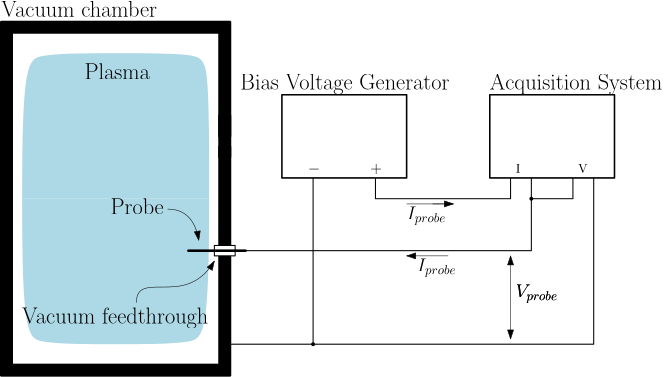
\includegraphics[width=3.4in]{lpms}
	\caption{General layout of a Langmuir probe acquisition system.}
	\label{fig1}
\end{figure}

A representative example of large-scale cold-plasma diagnostics is the Megavolt ITER Injector and Concept Advancement (MITICA), illustrated in Fig.~\ref{fig2}. MITICA is the full-scale prototype of the Neutral Beam Injector (NBI) for the International Thermonuclear Experimental Reactor (ITER) \cite{Toigo}. Installed at the PRIMA test facility in Padua, Italy, it is designed to demonstrate full-performance operation of the ITER neutral beam system, including the generation and acceleration of negative ion beams up to \measure{1}{MeV}. Plasma monitoring in MITICA relies on an extensive network of electrostatic probes distributed along the beam line, comprising a total of 212 measurement points located in the Neutralizer, Residual Ion Dump (RID), and Calorimeter. These diagnostics operate in multiple configurations, including Single and Double Langmuir Probe modes, and provide measurements of floating potential, electron temperature, plasma density, beam profiles, and secondary electron emission processes \cite{SPAGNOLO}. The large number of distributed measurements, together with the need for synchronized operation and flexible probe configurations, introduces significant challenges in terms of bias generation, data acquisition, and overall system scalability.



\begin{figure}[t]
	\centering
	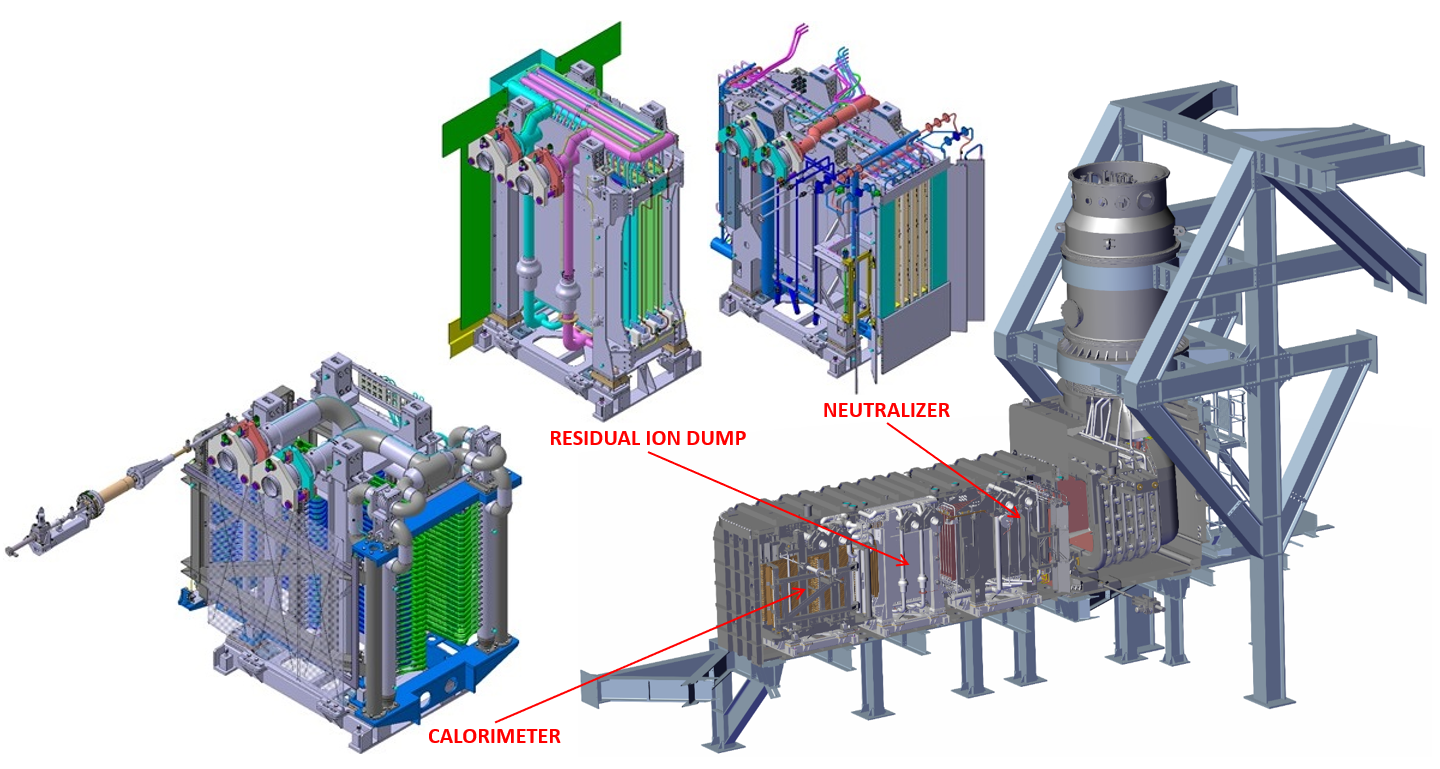
\includegraphics[width=3.4in]{MITICA3}
	\caption{MITICA design. The three components at the bottom of the schematic identifies the locations designated for probe installation.}
	\label{fig2}
\end{figure}

\begin{table}[t]
	\centering
	\footnotesize
	\renewcommand{\arraystretch}{1.5}
	\caption{Measurement ranges and relative resolution requirements.}
	\label{tab:meas_ranges}
	\begin{tabular}{c|c|c}
		\toprule
		\makecell{Measurement Range} & \makecell{Minimum \\resolution} & \makecell{Maximum residual \\r.m.s. noise} \\
		\midrule
		
		\multicolumn{3}{c}{\textit{Voltage measurements}} \\
		\midrule
		$\pm 100\,\mathrm{V}$ & $50\,\mathrm{mV}$ & $15\,\mathrm{mV}$ \\
		\midrule
		
		\multicolumn{3}{c}{\textit{Current measurements}} \\
		\midrule
		$\pm 1\,\mathrm{mA}$   & $0.5\,\mu\mathrm{A}$  & $0.15\,\mu\mathrm{A}$ \\
		$\pm 10\,\mathrm{mA}$  & $5\,\mu\mathrm{A}$    & $1.5\,\mu\mathrm{A}$ \\
		$\pm 100\,\mathrm{mA}$ & $50\,\mu\mathrm{A}$   & $15\,\mu\mathrm{A}$ \\
		$\pm 1\,\mathrm{A}$    & $500\,\mu\mathrm{A}$    & $150\,\mu\mathrm{A}$ \\
		\bottomrule
	\end{tabular}
\end{table}

Recent developments have addressed scalability limitations through the adoption of FPGA-based electronics. An example is the MAST-Upgrade Langmuir probe system, where dedicated control modules based on Xilinx Zynq devices provide arbitrary bias waveform generation and synchronized acquisition of voltage and current measurements from multiple probes \cite{Ryan}. Whereas this approach significantly improves scalability with respect to conventional laboratory instrumentation, the biasing and acquisition functions remain partially centralized and rely on multiplexed probe operation.

To address these challenges, this work presents EPICA (Electrostatic Probe Integrated Conditioning and Data Acquisition module), an integrated platform that combines power supply, control, and data acquisition functionalities for large Langmuir probe arrays. Unlike conventional systems based on centralized COTS instrumentation, EPICA embeds the probe biasing stage directly within each acquisition module. This approach improves scalability, reduces wiring complexity, and increases modularity, making the system better suited for high-density probe deployments.

EPICA is built on a high-performance hardware and software framework fully compatible with the ITER Control, Data Access and Communication (CODAC) system. The platform is designed to operate across a wide range of plasma conditions, covering electron densities from fractions of \measure{10^{15}}{m^{-3}} to \measure{10^{18}}{m^{-3}}, electron temperatures ranging from \measure{1}{eV} to \measure{10}{eV}, multiple probe configurations, and real-time data processing.

The proposed architecture supports synchronized operation across multiple distributed racks while satisfying the measurement resolution and noise requirements summarized in Table~\ref{tab:meas_ranges}. The requirements reported in Table~\ref{tab:meas_ranges} were derived from the expected plasma parameters and measurement accuracy targets defined for MITICA operation.

The main contributions of this work are threefold: (i) the development of a fully integrated probe-level biasing and acquisition module for high-density Langmuir probe arrays; (ii) a modular rack-based architecture scalable to large numbers of probes while maintaining synchronization; and (iii) a hardware and software implementation based on System-on-Module (SoM) technology and real-time frameworks enabling deterministic acquisition and processing in fusion-relevant plasma environments.

This paper is organized as follows. Section~\ref{secII} describes EPICA system architecture; Section~\ref{secIII} details the integrated polarization and acquisition module; Section~\ref{secIV} presents the software integration; Section~\ref{secV} reports the experimental validation; Section~\ref{secVI} discusses the results and Section~\ref{secVII} concludes the paper.